\documentclass[11pt]{article}
% Defining all packages that are used in this document
\usepackage[utf8]{inputenc}
\usepackage[english]{babel} % Change this to norwegian if report is written in norwegian
\usepackage{amsmath}   % Package for math files
\usepackage{parskip}   % No indent, but instead paragraphs
\usepackage{graphicx}  % Place figures
\usepackage{caption}   % Place captions in tables and figures
\usepackage{subcaption}% 
\usepackage{subfiles}  % 
\usepackage[T1]{fontenc} 
\usepackage[euler]{textgreek} % To get greek letters as we know them
\usepackage{amssymb}   % 
\usepackage{placeins}  % \FloatBarrier so figures can't float beyond some point in text
\usepackage{fullpage}  % Uses more of the page
\usepackage{float}     % Able to make figures and tables float \begin{figure}[H] to keep them HERE
\usepackage[version=4]{mhchem} % \ce{} to write chemical eq.
\usepackage{siunitx}   % Ex: \si{\meter\per\square\second}
\usepackage{booktabs}  % Behind-the-scenes optimization of tables. \toprule, \midrule, \bottomrule
\usepackage{hyperref}  % Ability to click on references like equations, figures, sections etc. \ref{eq:my_eq} clickable
\hypersetup{
    colorlinks,
    citecolor=black,
    filecolor=black,
    linkcolor=black,
    urlcolor=black
}
\usepackage[autolinebreaks,useliterate,numbered]{mcode} % Ability to paste smooth MATLAB code

\newcommand{\figref}[1]{\figurename~\ref{#1}} %Nice reference to figures
%\linespread{1.5}
\renewcommand{\baselinestretch}{1.5}
\title{
    Experiment B\\
    Flow meters
    }
\author{
	Jiaqi, Yao.%\footnote{jy431@exeter.ac.uk}
}
\date{
    26 October, 2022
}

\begin{document}
\maketitle
%\begin{abstract}
%    This section should contain a short and concise way of describing all parts of the report. It should be a summary of the introduction, what has been done and what you have found.
%\end{abstract}
\pagenumbering{gobble} % Turn off page numbering
%\newpage
%\tableofcontents
%\newpage
\pagenumbering{arabic} % Turn on normal pagenumbering
%%%%%%%%%%%%%%%%%%%%%%%%%%%%%%%%%%%%%%%%%%%%%%%%%%%%%%%%%%
% Main contents - Do NOT write your text in main.tex! Use                     the tex files in the folders below
\section{Introduction}
\label{sec:introduction}
\FloatBarrier % Now figures cannot float above section title
This section should concentrate on what has previously been done in the field of research, so that it incentivizes the experiment. Why is there a need to gain knowledge on this specific field, and what motivates you to conduct the experiment? Often the introduction lists up a lot of historical facts and previous reports, and then it presents the topic for the report. The section is here for make a smooth transaction over to what you will be covering later on. It may be a good idea to present figures to back up your claims as done in figure \figref{fig:intro_co2}. Never post jpg, jpeg or bmp files in figures, but try to stick to png or eps format. Even though you have presented the figure in this text, the caption on the figure must still be able to present the information alone independent of this text! It should also be placed BENEATH the actual figure. Also remember to always write passive, i.e. no personal pronouns (I, you, he, we, you, they). It is recommended that you learn Mendeley for managing your references that has great support in Sharelatex. Upper left corner $\rightarrow$ Menu $\rightarrow$ Mendeley inserts your whole personal library into the document, so that you don't have to worry about formatting your references correctly. \LaTeX does that for you.
% Historical chart of CO2 emissions
\begin{figure}[htb] % Here, top, bottom priority list
    \centering
    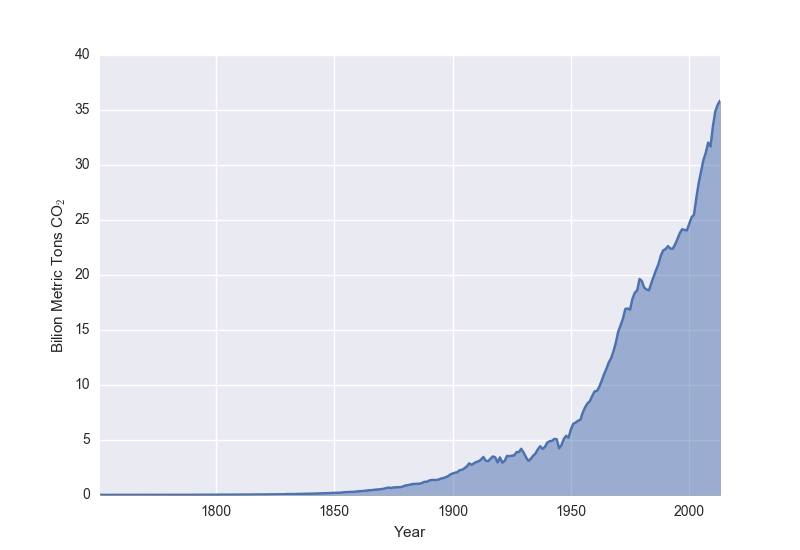
\includegraphics[scale=0.45]{Introduction/figures/Historic_CO2_Emission}
    \caption{This text should be able to stand alone independent of text outside figure!}
    \label{fig:intro_co2}
\end{figure}
\section{Theory}
%\label{sec:problem_description}



\section{Method}

As can be seen above,  
It need to measure the trajectory of jet and different head between 1 and 2.  

The head difference between 1 and 2 can be easily measured by tools such as a ruler.
For the trajectory of the water jet of 2, 
adjusting the needle mounted on the back plate so that its bottom point is as close as possible 
to the upper edge of the jet, and tighten the screws.

Next, attach a sheet 
of paper to the back-board between the needle and board,
and make sure it is horizontal and secure.

As you can see in the \autoref{fig:demo},
Set up the same coordinate system on the attachment sheet, 
and then measure the x and y distance between each marker point to get table 
\ref{t1}.

In order to ensure the accuracy of the data, 
four data sets were measured by using two different orifice diameters and 
two different heights.

In experiment A2, a measuring cylinder is a good tool to measure the flow rate of water. 
First, prepare an empty measuring cylinder and collect the water jet from position 2. 
When the measuring cylinder starts to receive water, press the stopwatch to start timing. 
Wait for a period of time until the measuring cylinder exceeds 800 ml, 
then stop collecting water and stop timing.

















\section{Results}
\label{sec:results}

The experiment data is shown in the following table.

\begin{table}[h]
    \centering
    \scalebox{0.9}{
    \begin{tabular}{c|cccccccccccccc}
    \toprule
    No. &Flowrate& $h_1$   & $h_2$   & $h_3$  & $h_4$  & $h_5$  & $h_6$  & $h_7$  & $h_8$&$V_1$(l)  & $T_1$(s)&  $V_2$(l)   & $T_1$(s)& $Q_{average} $= $\frac{V}{T}$ (L/s)  \\ 
    \midrule
    1&5(L/min)  & 220 & 203 & 211 & 209 & 155 & 155 & 145 & 149&6  & 63    & 7  & 70.06 &  0.097576 \\
    2&10 (L/min)& 248 & 199 & 228 & 220 & 164 & 165 & 132 & 143&11 & 63    & 11 & 64.47 &  0.172613 \\
    3&15 (L/min)& 294 & 187 & 255 & 240 & 175 & 180 & 106 & 130&15 & 60.25 & 16 & 63.03 &  0.251405 \\
    4&20(L/min) & 355 & 160 & 300 & 270 & 197 & 205 & 68  & 117&22 & 65    & 22 & 64    &  0.341106 \\ 
    \bottomrule
    \end{tabular}}

    (Unit of h: mm)
    \caption{Recording of pressure tubes}
    \label{Bt2}
\end{table}

%\begin{table}[h]
%    \centering
%    \scalebox{0.8}{
%\begin{tabular}{ccccc}
%    \toprule
%    $V_1$(l)  & $T_1$(s)&  $V_2$(l)   & $T_1$(s)& $Q_{average} $= $\frac{V}{T}$ (L/s)  \\
%    \midrule
%6  & 63    & 7  & 70.06 &  0.097576 \\
%11 & 63    & 11 & 64.47 &  0.172613 \\
%15 & 60.25 & 16 & 63.03 &  0.251405 \\
%22 & 65    & 22 & 64    &  0.341106 \\
%    \bottomrule
%\end{tabular}}
%\caption{Recording of real flow}
%\label{Bt3}
%\end{table}






































%All your results should be presented by now, and all that remains is that you discuss them. You should always be critical of your results, and if they are not in correspondence with your theory presented in section \ref{sec:problem_description} this should be elaborated on! Why is there a mismatch between those two? What could have gone wrong and what do these non-correspondences imply? If there are undiscussed results, do not neglect them! It is easily seen and it doesn't look good in the report. Good reports really stand out from bad ones in this section and you can shine through if you have a well thought through reflection here.
\section{Analysis}
\label{sec:analysis}
\subsection{Regression analysis}
For experimentA1,
Plot a scatter chart with $\sqrt{gh}$ as the horizontal coordinate 
and x as the vertical coordinate based on the data from Table \ref{t1}.
And a regression analysis and linear fit was performed on the data, 
as shown in \autoref{ExperimentA1} and results in \autoref{table4}.

Take the average of 
the data and take it into equation \eqref{6} to get $C_v=\frac{slope}{2}$.
The final $C_v$ is 0.955.

For experiment A2, it is the same as experiment A1, with the horizontal 
coordinates replaced by $\sqrt{h}$ and the vertical coordinates replaced by Q
the data of regression analysis is in \autoref{ExperimentA2}
and results in \autoref{table5}.

Use equation \eqref{13} to caculate the $C_d=\frac{Slope}{A_0\sqrt{2g}}$
and the final $C_d$ is 0.615 (3mm)
and 0.8816 (6mm).

\begin{figure}[h]
    \centering
    \begin{minipage}[t]{0.49\textwidth}
        \centering
        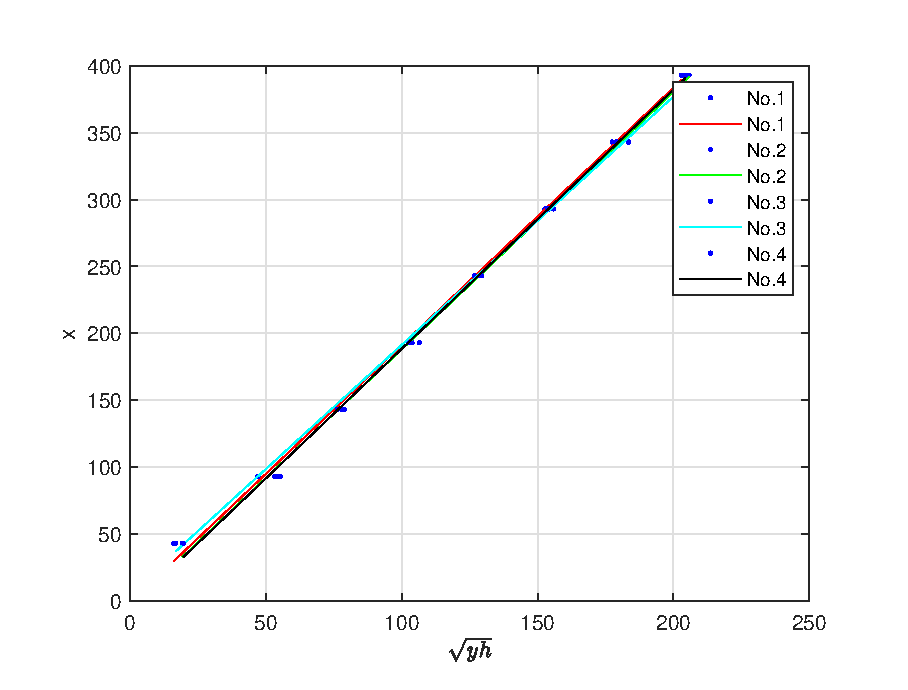
\includegraphics[width=1.12\linewidth]{Results/1.eps}
        \caption{ExperimentA1}
        \label{ExperimentA1}
        (Unit:mm)
    \end{minipage}
    \begin{minipage}[t]{0.49\textwidth}
        \centering
        \includegraphics[width=1.12\linewidth]{Results/A2.eps}
        \caption{ExperimentA2}
        \label{ExperimentA2}
       (Unit:$\sqrt{m}$ and $m^3/s$)
    \end{minipage}
\end{figure}

\begin{minipage}{\textwidth}
    \centering
\begin{minipage}[t]{0.49\textwidth}
    \makeatletter\def\@captype{table}
    \centering
    \scalebox{0.9}{
    \begin{tabular}{l|ll} 
        \hline
            & Slope    & R-square \\ \hline
        1 & 1.923 & 0.9968   \\
        2 & 1.923 & 0.9976   \\
        3 & 1.855 & 0.9985   \\
        4 & 1.936 & 0.998   \\ \hline          
    \end{tabular}} 
    \caption{result of A1 regression analysis}
    \label{table4} 
\end{minipage}
\begin{minipage}[t]{0.49\textwidth}
    \makeatletter\def\@captype{table}
    \centering
    \scalebox{0.9}{
    \begin{tabular}{l|ll}
        \hline
            & Slope    & R-square \\ \hline
        3mm & 0.00001924 & 0.9955   \\
        6mm & 0.0001103 & 0.9811   \\ \hline
        \end{tabular}}
    \caption{result of A2 regression analysis}
    \label{table5} 
\end{minipage}
\end{minipage}


%\begin{table}[h]
%    \centering
%    \begin{tabular}{l|ll}
%    \hline
%        & Slope    & R-square \\ \hline
%    3mm & 0.00001924 & 0.9955   \\
%    6mm & 0.0001103 & 0.9811   \\ \hline
%    \end{tabular}
%    \caption{result of A2 regression analysis}
%    \label{table5}
%\end{table}

\subsection{Error analysis}

$\bullet$ Inaccurate recording of water trajectory to the sheet 
due to not looking horizontally at the top point of the needle.

$\bullet$ Inaccurate calculation of the flow rate due to residual 
water in the measuring cylinder.

$\bullet$ When calculating the flow rate, errors caused by the stopwatch timing not being fully 
synchronised with the water collection time.

\FloatBarrier
\section{Conclusion}
\label{sec:conclusion}
%The conclusion should, as the abstract, wrap up what you have found in the experiment. It should state what you have done and what you have found. The conclusion should only state what is obvious from the discussion in section \ref{sec:results}; no new information should arise here. The conclusion is the first place the reader will go looking if he wants to get an overview of the report. If it is interesting, he might read the rest. Be sure that the conclusion is short and concise, but do not omit important information. You have one shot at presenting your results: if you have done excellent work at the lab it doesn't matter if you are unable to present the results in an appealing way. The report is your only way of communicating and presenting your hard work.

From the results of the regression analysis, 
the R-square value of both experiment A1 and A2 are larger than 0.98, 
which demonstrates a strong linear correlation between the x and y axes.

In addition, from the above it follows that $C_v = 0.955$,$C_d=0.615$(3mm),$C_d=0.8816$
(6mm). Both of the coefficient are less than 1.This satisfies the hypothetical conditions.

Therefore, the data from the regression analysis is valid.


%\section*{List of Symbols}
\begin{table}[H]
\centering
\begin{tabular}{lll}
 \toprule
  \textbf{Symbol}   &\textbf{Unit}      &\textbf{Explanation}\\
  \midrule
    n               & \si{\mole}        & Amount of substance \\
    m               & \si{\kilo\gram}   & Mass \\
    H               & \si{\kilo\joule\per\mole} & Molar enthalpy \\
    S               & \si{\joule\per\kelvin\per\mole}   & Molar entropy \\
    G               & \si{\kilo\joule\per\mole} & Gibbs free energy \\
    A               & \si{\kilo\joule\per\mole} & Helmholtz free energy \\
  \bottomrule
  \end{tabular}
\end{table}

%%%%%%%%%%%%%%%%%%%%%%%%%%%%%%%%%%%%%%%%%%%%%%%%%%%%%%%%%%
% Bibliography
\newpage
\bibliographystyle{IEEEtran}
\bibliography{mendeley.bib}
%%%%%%%%%%%%%%%%%%%%%%%%%%%%%%%%%%%%%%%%%%%%%%%%%%%%%%%%%%
% Appendix
%\appendix
%\pagenumbering{roman}
%\section{First Appendix}
\label{app:first_appendix}
%\section{Second Appendix}
%\section{Third Appendix}
\end{document}
